\chapter{Introdução}

Neste capítulo, apresenta-se uma descrição inicial do problema abordado, juntamente com os principais desafios e motivações para a realização desta pesquisa. Na Seção \ref{subsec:contextualização}, contextualiza-se o cenário do mercado de ações e os acontecimentos que contribuíram para o seu desenvolvimento. Em seguida, na Seção \ref{subsec:motivação}, são apresentadas a motivação e a relevância do estudo. Na Seção \ref{subsec:objetivo}, descreve-se o objetivo geral do trabalho, juntamente com seus objetivos específicos. Por fim, na Seção \ref{subsec:organização}, é apresentada a estrutura deste trabalho, destacando como as seções estão organizadas.


\section{Contextualização}
\label{subsec:contextualização}
Os primeiros registros de mercados financeiros similares aos contemporâneos, surgiram no século XVII na Holanda, com a criação da Bolsa de Valores de Amsterdam, onde comerciantes e investidores se reuniam para negociar ações de empresas da Companhia das Índias Orientais \cite{french2006dutch}. Desde então, o mercado de ações evoluiu e se expandiu para outros países, tornando-se uma importante fonte de financiamento para empresas e um meio para os investidores obterem lucros.

Com a expansão e grande aceitação do modelo financeiro, iniciou-se o mercado de índices no final do século XIX nos Estados Unidos, quando Charles H. Dow, fundador de \textit{The Wall Street Journal}, deu nome ao primeiro índice de ações \cite{Richard1986}, conhecido como \ac{DJIA}. O \ac{DJIA} foi criado em 1986 com o intuito de acompanhar a performance do mercado de ações e fornecer uma medida do desempenho das empresas, aplicando uma média ponderada dos preços das ações de 12 empresas industriais americanas \cite{John_Dow}. 
Em seguida, outros índices de ações foram criados em todo o mundo, como o FTSE 100 no Reino Unido, o Nikkei no Japão, o S\&P 500 nos Estados Unidos e o Ibovespa no Brasil. Guiando para o que se conhece nos dias atuais, em que há diversos índices de ações que representam diferentes setores da economia, indústrias e países.

Ao longo da história, os índices de ações surgiram como uma forma de investimento, o que levou ao desenvolvimento do mercado de índices \cite{John2000}. Esse mercado permite que os investidores comprem e vendam um conjunto de ações representadas por um índice, em vez de adquirir ações individuais. Essa forma de investimento é conhecida como \ac{ETFs} e tem se tornado popular devido à diversificação, custos reduzidos e facilidade de negociação que oferece \cite{ben2017exchange}. Os \ac{ETFs} permitem que os investidores tenham exposição a um portfólio diversificado de ativos por meio de uma única transação, proporcionando benefícios em termos de redução de riscos e acesso a diferentes setores e mercados \cite{gad2019diversification}.

A teoria financeira subjacente ao mercado de índices conhecida como eficiência de mercado, afirma que os preços dos ativos financeiros refletem todas as informações disponíveis publicamente \cite{Paul_Proof}. Isso significa que é improvável obter lucros anormais de forma consistente baseado apenas em informações públicas \cite{MALKIEL2003}. Tal ocorrência é devido a grande procura de informações por parte dos investidores para obter vantagem competitiva no mercado, o que leva a uma rápida incorporação de informações aos preços dos ativos financeiros \cite{Fama_EFFICIENT}. 
No entanto, há críticas à teoria da eficiência de mercado, uma vez que existem evidências empíricas de que os preços das ações podem ser influenciados por fatores emocionais e comportamentais, como o comportamento de manada e a aversão à perda \cite{Shiller2000}. Possibilitando a ineficiências de mercado e oportunidades de investimento para os investidores que são capazes de identificá-las.

Em um estudo realizado por \citeonline{CAJUEIRO2004521}, investigou-se os coeficientes de \textit{Hurst} das séries de preços de ações de países desenvolvidos e emergentes com o objetivo de encontrar correlações entre as variações passadas e os estados futuros. O coeficiente de \textit{Hurst} é utilizado para medir a dependência de longo prazo em uma série temporal, onde um valor igual a 0,5 indica uma série temporal aleatória, em que os valores passados não possuem influência sobre os valores futuros. 
Os resultados desse estudo indicaram que os coeficientes de \textit{Hurst} das séries de países desenvolvidos estavam próximos de 0,5, o que é consistente com a hipótese de mercado eficiente \cite{mussa2010hipotese}. Por outro lado, os valores obtidos para os países emergentes se distanciaram mais desse valor, sugerindo que os mercados emergentes são menos eficientes que os mercados desenvolvidos.
Este acontecimento pode ser explicado por diversos fatores, como a menor liquidez e transparência dos mercados emergentes, a menor qualidade das informações disponíveis, a presença de assimetrias de informação e a maior aparição de investidores não informados \cite{BARBERIS1998307}. Resultando em desvios sistemáticos dos preços em relação ao seu valor justo, e consequentemente a existência de oportunidades para os investidores obterem retornos consideráveis de forma consistente. 

A busca por estratégias menos arriscadas e com maior potencial de retorno originou diversos modelos aplicáveis ao mercado financeiro, os quais posteriormente contribuíram para a exploração de evidências significativas que contestam a teoria de mercado eficiente \cite{Paul_Proof}. Esses modelos são baseados em:
\begin{itemize}
    \item \ac{AT}: essa análise originou-se no ocidente por volta de 1900, quando Charles H. Dow, publicou uma série de editoriais sobre métodos de especulação com ações \cite{MORRIS1994}. Tais métodos surgiram com o objetivo de indicar padrões e tendências de mercado a partir de observações gráficas, baseado-se em informações passadas dos ativos financeiros. 
    \item \ac{AF}: foi desenvolvida ao longo do século XX por Benjamin Graham \cite{GRAHAM1934} com o objetivo de avaliar o preço justo (valor real) de ações que se respalda na expectativa de resultados futuros da empresa \cite{CAVALCANTE2005}. Tal análise se dá devido ao preço da ação na bolsa ser ocasionado de uma média de emoções e expectativas dos vendedores e compradores embutidos nesse meio. 
    \item \ac{AQ}: surgiu nas décadas de 1940 e 1950, impulsionada pelos primeiros computadores eletrônicos que permitiam processar grandes quantidades de dados de maneira rápida e eficiente \cite{TING2015}. O foco principal dessa abordagem é o uso de modelos matemáticos complexos para identificar padrões e tendências no mercado.   
    \item \ac{AS}: surgiu posteriormente ao desenvolvimento teórico da linguística computacional e da \ac{IA}, em meados da década de 1960. Porém, começou a ganhar destaque somente na década de 1990 com a chegada de programas de processamento de linguagem natural capazes de identificar a polaridade dos sentimentos expressos em textos \cite{SENTIMENTALWILLSON}. Desde então, tal abordagem vem sendo utilizada em diferentes contextos, sendo um deles o mercado de ações e índices, focado em realizar previsões sobre a direção dos preços \cite{SENTIMENTAL2, SENTIMENTAL1, SENTIMENTAL3}. 
\end{itemize}

Como consequência, surgiram posteriormente modelos baseados em \ac{IA} que combinam \ac{AT}, \ac{AF}, \ac{AQ} e \ac{AS}, com o objetivo de realizar operações mais precisas e assertivas no mercado de ações \cite{agrawal2022stock}. Esses modelos incorporam algoritmos de aprendizado de máquina, permitindo a análise de grandes volumes de dados e o reconhecimento de padrões complexos \cite{vadlamudi2017stock}.

\section{Motivação e Relevância}
\label{subsec:motivação}
O crescente interesse e participação de pessoas físicas no mercado financeiro têm sido observados em todo o mundo. Em uma análise realizada pela Bolsa de Valores de Nova York, constatou-se que a globalização dos mercados financeiros e o aumento da renda das famílias em países em desenvolvimento são alguns dos principais fatores que impulsionam essa tendência \cite{KANIEL_Individual}. Além disso, a facilidade de acesso à informação e o uso cada vez maior de tecnologias financeiras, como aplicativos de investimento, têm contribuído significativamente para o aumento da participação de pessoas físicas na bolsa de valores \cite{UNCTAD2020}. Essas mudanças refletem uma maior democratização do mercado financeiro, permitindo que mais pessoas tenham a oportunidade de investir e se envolver ativamente no processo de tomada de decisões financeiras.

\begin{figure}
    \caption{Porcentagem de pessoas por país que investem em ações.}
      \centering
      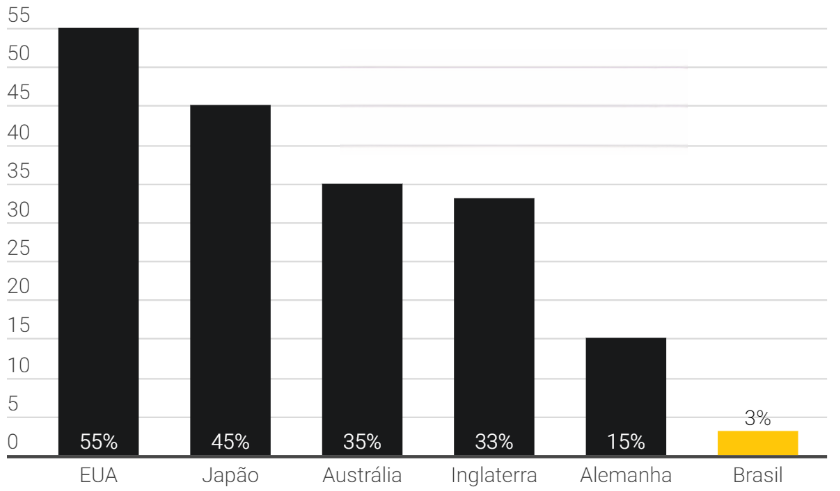
\includegraphics[width=.8\linewidth]{InvestingActionXP.png} 
      
      Fonte: Adaptado de \citeonline{XP:2023}.
    \label{fig:investPerCountry}
\end{figure}

O estudo realizado pela XP Investimentos \cite{XP:2023} revela que o número de pessoas físicas investindo em ações está diretamente relacionado à estabilidade do mercado e à qualidade de vida nos países analisados. A Figura \ref{fig:investPerCountry} ilustra essa relação, confirmando que países com maior estabilidade econômica e política, como Estados Unidos e Japão, possuem uma maior proporção de investidores individuais. Por outro lado, nos mercados emergentes, o crescimento do número de investidores é mais acentuado devido à entrada de novos participantes. Esse fenômeno também tem sido observado na bolsa de valores brasileira (B3), com um aumento significativo no número de investidores pessoa física nos últimos anos. Em 2020, houve um acréscimo de mais de 2,8 milhões de investidores individuais em relação ao ano anterior, representando um crescimento de 93,7\% em relação a 2019 \cite{B3:2023}. Esses incrementos podem ser visualizados na Figura \ref{fig:PessoasActionsXP}, o que e reflete diretamente na posição total dos ativos como pode ser observado na Figura \ref{fig:ValorActionXP}.

\begin{figure}
     \centering
     \caption{Dados da bolsa de valores brasileira}
     \begin{subfigure}[b]{0.48\textwidth}
         \centering
         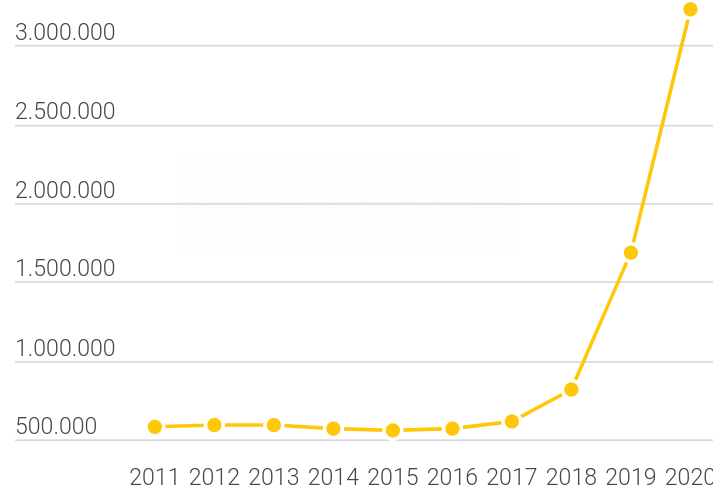
\includegraphics[width=\textwidth]{PessoasActionsXP}
         \caption{Pessoas físicas cadastradas na Bolsa de Valores}
         \label{fig:PessoasActionsXP} 
     \end{subfigure}
     \hfill
     \begin{subfigure}[b]{0.48\textwidth}
         \centering
         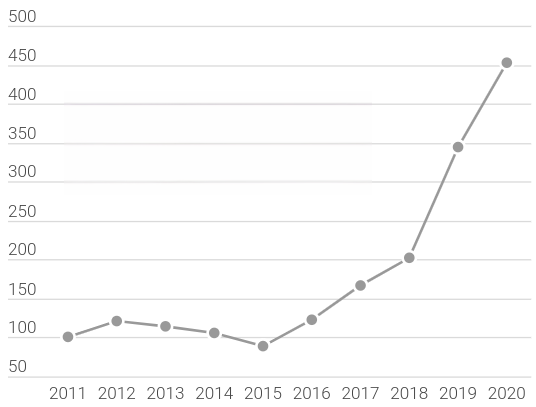
\includegraphics[width=\textwidth]{ValorActionXP}
         \caption{Posição total em R\$ bilhões dos investidores pessoa física na Bolsa}
         \label{fig:ValorActionXP}
     \end{subfigure}

     Fonte: Adaptado de \citeonline{XP:2023}.
\end{figure}

\citeonline{Gonzalo_Estimation1} mostraram que a previsão de séries temporais pode ser uma ferramenta útil na especulação de retornos de ações, com resultados significativos e positivos \cite{Gonzalo_Estimation2}. Esta técnica tem sido explorada há décadas e é uma área de grande interesse para investidores em todo o mundo, uma vez que pode ser utilizada para melhorar a tomada de decisões no ato do investimento, mitigar riscos e gerar lucros. Sendo assim, é possível realizar o uso de modelos de \ac{IA}, aplicados a tarefas de previsão de sentido e/ou valor de ativos financeiros. Isso se dá devido à sua alta capacidade de identificar rapidamente padrões dificilmente observados por seres humanos e de fornecer dados futuros com maior probabilidade de acontecimento, respaldados em padrões previamente computados \cite{Jerzy_Deep}.

Na literatura, várias pesquisas têm sido realizadas com o objetivo de prever valores futuros de ações. Esses estudos exploram diferentes abordagens, incluindo modelos matemáticos lineares que buscam identificar oportunidades em desvios da hipótese de mercado eficiente \cite{Charlene}. Esses modelos lineares utilizam equações e métodos estatísticos para analisar os dados históricos e identificar padrões que possam sinalizar movimentos futuros no mercado financeiro.

Adicionalmente, também são aplicados diferentes modelos de aprendizado de máquina na previsão de valores futuros de ações, conforme mencionado por \citeonline{Ciniro_Econometric} e \citeonline{Leonardo_Comparative}. Esses modelos utilizam algoritmos e técnicas para aprender com dados históricos e fazer previsões com base em padrões identificados.
Além disso, são exploradas abordagens híbridas que combinam vários modelos de previsão em um comitê, buscando obter um modelo final mais robusto e assertivo \cite{Jerzy_Deep}. 

Com o avanço da tecnologia e o crescente interesse dos investidores individuais, torna-se cada vez mais importante explorar e desenvolver métodos que possam ajudar na previsão de valores futuros de ações. Nesse contexto, o presente trabalho tem como objetivo principal contribuir para esse campo de pesquisa, explorando diferentes modelos de predição e aplicando-os a uma abordagem de comitê (\textit{ensemble}). A proposta é construir um sistema de recomendação de investimentos que seja capaz de fornecer \textit{insights} valiosos para os investidores, auxiliando-os na tomada de decisões financeiras mais informadas. 

\section{Objetivo}
\label{subsec:objetivo}
\subsection{Objetivo Geral}
\label{subsubsec:objetivo_geral}
O objetivo geral deste trabalho é aplicação de técnicas de \ac{IA} para previsão e recomendação de investimentos no mercado financeiro.

\subsection{Objetivos Específicos}
\label{subsubsec:objetivo_especifico}
Para alcançar o objetivo geral, propõe-se os seguintes objetivos específicos:

\begin{itemize}
    \item revisar a literatura sobre mercado financeiro e técnicas de \ac{IA} aplicadas a tarefas de previsão e classificação;
    \item propor e implementar uma abordagem para a previsão de valores e previsão de sentido de variação;
    \item avaliar o desempenho do modelo proposto;
    \item propor e implementar uma abordagem para realizar a recomendação de compra e venda de ativos;
    \item avaliar os resultados da abordagem proposta.
\end{itemize}

\section{Organização do Trabalho}
\label{subsec:organização}
A fim de facilitar a compreensão do trabalho proposto, o estudo foi dividido em três seções que introduzem gradualmente os conceitos necessários para entender a proposta. Neste capítulo, são apresentados o contexto do problema, as motivações e os objetivos gerais e específicos para a realização da proposta. Em seguida, o Capítulo \ref{cap:trabalhos_relacionados} aborda estudos relacionados às técnicas de previsão de valores no mercado financeiro. No Capítulo \ref{cap:abordagem_proposta}, é apresentada uma abordagem para a previsão de valores em series temporais financeira e recomendações de investimento.

\newpage

